\documentclass[final,t]{beamer}
\mode<presentation>
{
%  \usetheme{Warsaw}
%  \usetheme{Aachen}
%  \usetheme{Oldi6}
%  \usetheme{I6td}
  \usetheme{I6dv}
%  \usetheme{I6pd}
%  \usetheme{I6pd2}
}
% additional settings
\setbeamerfont{itemize}{size=\normalsize}
\setbeamerfont{itemize/enumerate body}{size=\normalsize}
\setbeamerfont{itemize/enumerate subbody}{size=\normalsize}

% additional packages
\usepackage{times}
\usepackage{amsmath,amsthm, amssymb, latexsym}
\usepackage{exscale}
%\boldmath
\usepackage{booktabs, array}
%\usepackage{rotating} %sideways environment
\usepackage[english]{babel}
\usepackage[latin1]{inputenc}
\usepackage[orientation=landscape,size=custom,width=200,height=120,scale=1.9]{beamerposter}
\listfiles
\graphicspath{{../graphics/}}
% Display a grid to help align images
%\beamertemplategridbackground[1cm]
 
\title{\huge Verification of the Neutron Mirror Capabilities in MCNPX via Gold Foil Measurements at the EIGER Instrument Beamline at the Swiss Spallation Neutron Source (SINQ) } %\thanks{Supported by Swiss National Science Foundation grant 200021\_150048/1}
\author{R.M. Bergmann, U. Filges, S. Forss, D. Reggiani, E. Rantsiou, T. Reiss, U. Stuhr, V. Talanov, M. Wohlmuther} %\thanks{ryan.bergmann@psi.ch}
\institute[PSI]{Paul Scherrer Institut, Villigen, Switzerland}
\date[May 7th, 2015]{May 7th, 2015}

% abbreviations
\usepackage{xspace}
\makeatletter
\DeclareRobustCommand\onedot{\futurelet\@let@token\@onedot}
\def\@onedot{\ifx\@let@token.\else.\null\fi\xspace}
\def\eg{{e.g}\onedot} \def\Eg{{E.g}\onedot}
\def\ie{{i.e}\onedot} \def\Ie{{I.e}\onedot}
\def\cf{{c.f}\onedot} \def\Cf{{C.f}\onedot}
\def\etc{{etc}\onedot}
\def\vs{{vs}\onedot}
\def\wrt{w.r.t\onedot}
\def\dof{d.o.f\onedot}
\def\etal{{et al}\onedot}
\makeatother




%%%%%%%%%%%%%%%%%%%%%%%%%%%%%%%%%%%%%%%%%%%%%%%%%%%%%%%%%%%%%%%%%%%%%%%%%%%%%%%%%%%%%%%%%%%%%%%%%%%%%%%%%%%%
%%%%%%%%%%%%%%%%%%%%%%%%%%%%%%%%%%%%%%%%%%%%%%%%%%%%%%%%%%%%%%%%%%%%%%%%%%%%%%%%%%%%%%%%%%%%%%%%%%%%%%%%%%%%
\begin{document}
\begin{frame}{} 
  \begin{columns}[t]
    \begin{column}{.3\linewidth}

      %%%%%%%%%%%%%%%%%%%%%%%%%%%%%%%%%%%%%%%%%%%%%%%%%%%%%%%%%%%%%%%%%%%%%%%%%%%%%%%%%%%%%%%%%%%%%%%%%%%%%%%%%%%%

      \begin{block}{Introduction}
        \begin{itemize}
        \item automatic sign language recognition system                                    %what
        \item \alert{necessary for communication} between deaf and
          hearing people
        \item \alert{continuous} sign language recognition,
          \alert{several} speakers, \alert{vision-based} approach, \alert{no
            special hardware}
        \item large vocabulary speech recognition (LVSR) system to
          obtain a textual representation of the signed
          sentences 
        \item evaluation of speech recognition techniques on \alert{publicly
          available sign language
          corpus}
        \end{itemize}
      \end{block}

      %%%%%%%%%%%%%%%%%%%%%%%%%%%%%%%%%%%%%%%%%%%%%%%%%%%%%%%%%%%%%%%%%%%%%%%%%%%%%%%%%%%%%%%%%%%%%%%%%%%%%%%%%%%%
      
      \begin{block}{Automatic Sign Language Recognition (ASLR)}
        \begin{columns}[T]
          \begin{column}{.49\linewidth}
            \begin{itemize}
            \item \alert{similar to speech recognition}: temporal sequences of images
            \item important features
              \begin{itemize}
              \item hand-shapes, facial expressions, lip-patterns
              \item orientation and movement of the hands, arms or body
              \end{itemize}
            \item HMMs are used to compensate time and amplitude variations of the signers\par
              \vskip2ex              
              \centerline{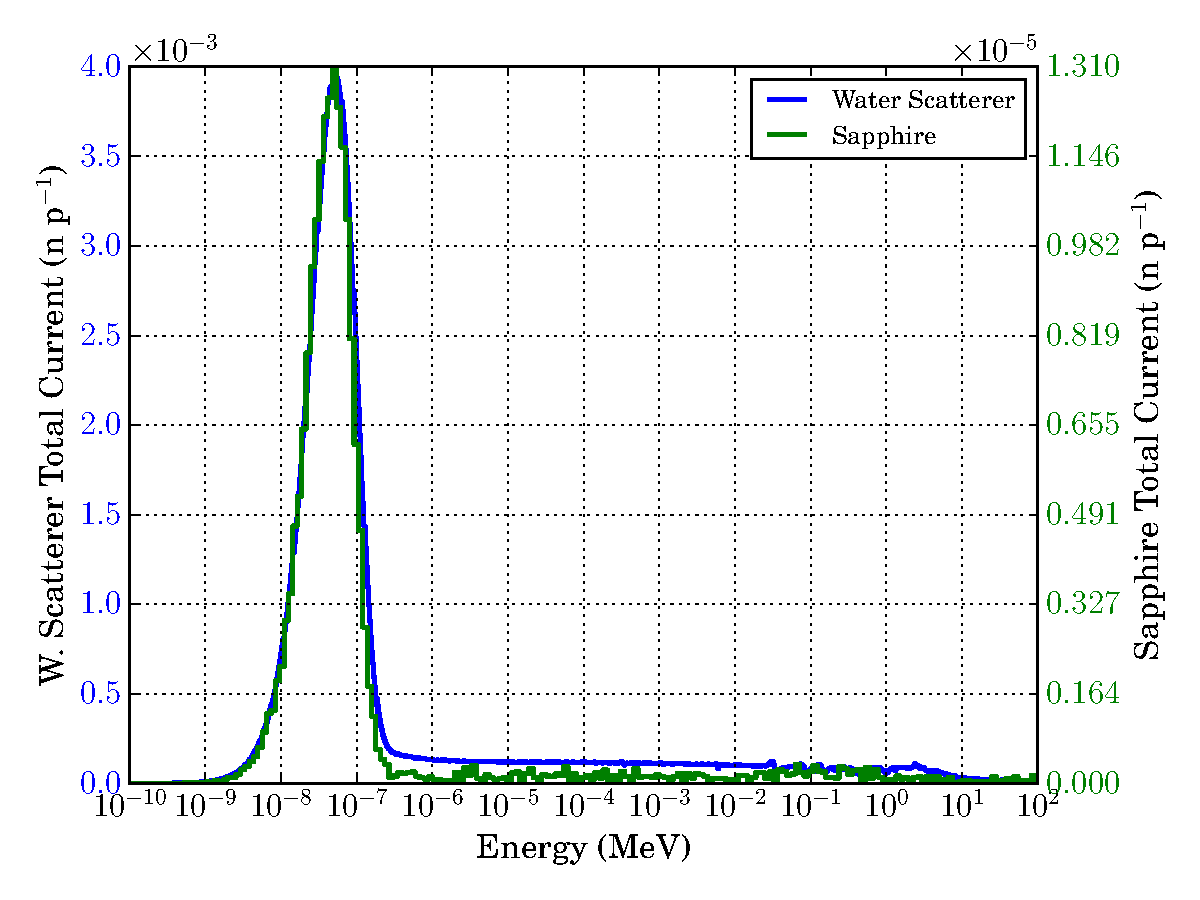
\includegraphics[width=.5\linewidth]{specs.pdf}}
            \end{itemize}
          \end{column}
          \begin{column}{.49\linewidth}
            \begin{itemize}
            \item \alert{goal:} find the model which best expresses the observation sequence
            \end{itemize}
            \vskip2ex
            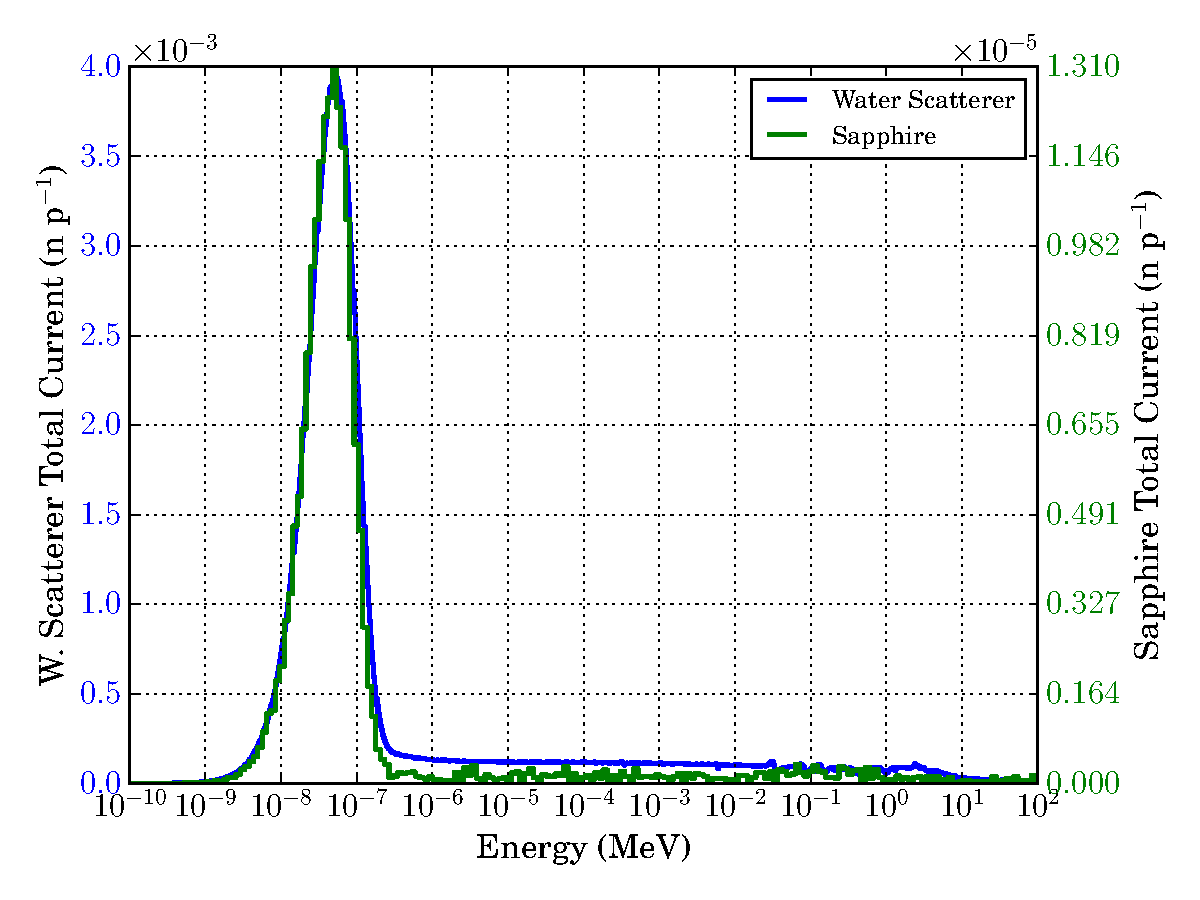
\includegraphics[width=\linewidth]{specs.pdf}
          \end{column}
        \end{columns}
      \end{block}

      %%%%%%%%%%%%%%%%%%%%%%%%%%%%%%%%%%%%%%%%%%%%%%%%%%%%%%%%%%%%%%%%%%%%%%%%%%%%%%%%%%%%%%%%%%%%%%%%%%%%%%%%%%%%
      \begin{block}{Experimental Setup}
        \begin{columns}[t]
          \begin{column}{.75\linewidth}
            \noindent{\hskip1cm\textbf{Database}}
            \begin{itemize}
            \item system evaluation on the RWTH-BOSTON-104 database
              \begin{itemize}
              \item \alert{201 sentences} (161 training and 40 test sequences)
              \item vocabulary size of \alert{104 words}
              \item 3 speakers (2 female, 1 male)
              \item corpus is annotated in glosses
              \end{itemize}
            \end{itemize}

            \vskip1ex            
            \noindent{\hskip1cm\textbf{Problems}}
            \begin{itemize}
            \item 26\% of the training data are \alert{singletons}
            \item simple sentence structure
            \item one out-of-vocabulary (OOV) words with whole-word models
            \end{itemize}

            \vskip1ex            
            \noindent{\hskip1cm\textbf{Differences in Comparison to ASR}}
            \begin{itemize}
            \item simultaneousness                       % multi-channel ... but unclear if necessary
            \item signing space                          % verb flexion, negation, ... 
            \item environment                            % cluttered background, clothes, lighting, ... different microphones in ASR?
            \item speakers and dialects                  % as in ASR 
            \item coarticulation and movement epenthesis % 
            \item silence                                % unclear as there might be no energy changes in signal but still information, e.g. holded signs
            \item whole-word models and sub-word units   % necessary for large-vocabulary systems
            \end{itemize}
          \end{column}

          \begin{column}{.25\linewidth}
            \vskip0ex
            %%%%%%%%%%%%%%%%%%%%%%%%%%%%%%%%%%%
            \centering    
            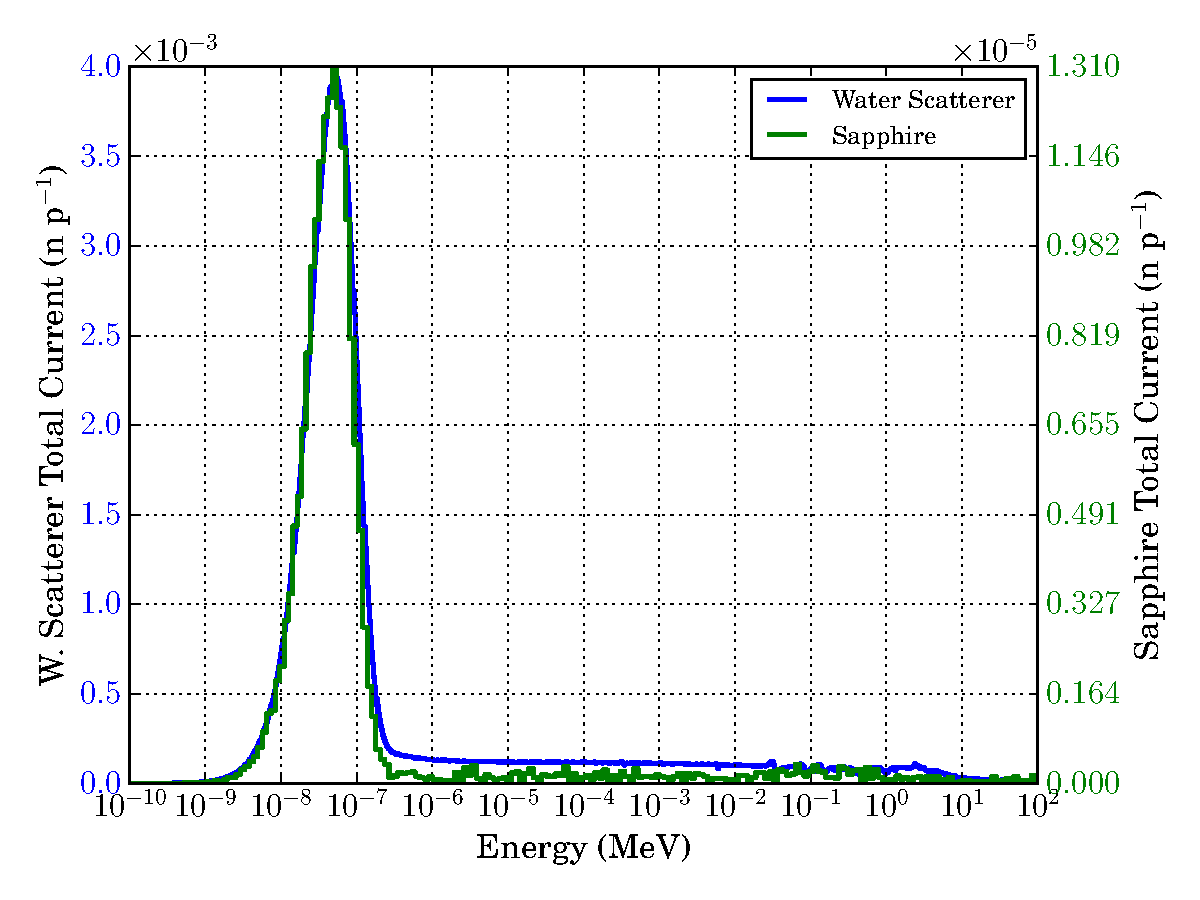
\includegraphics[width=0.7\linewidth]{specs.pdf}\\[1ex]
            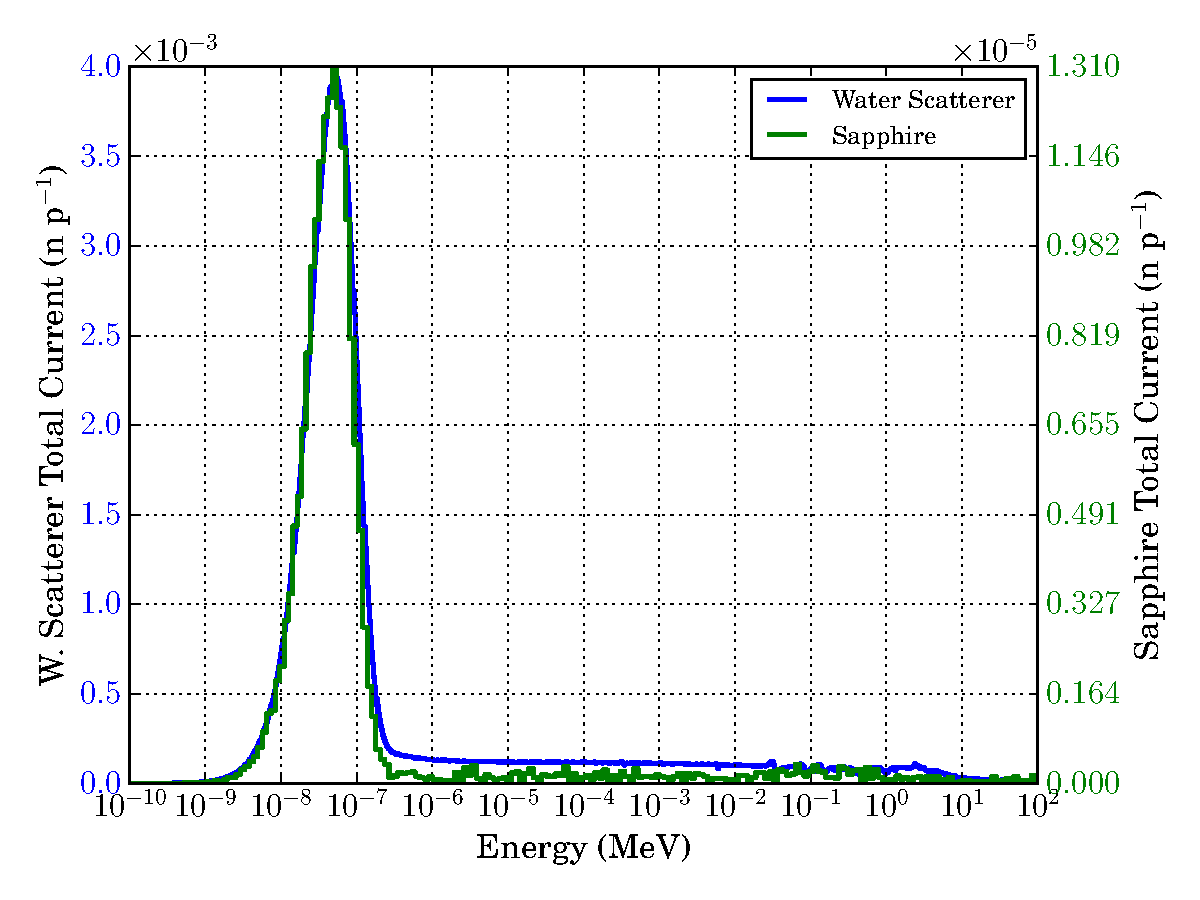
\includegraphics[width=0.7\linewidth]{specs.pdf}\\[1ex]
            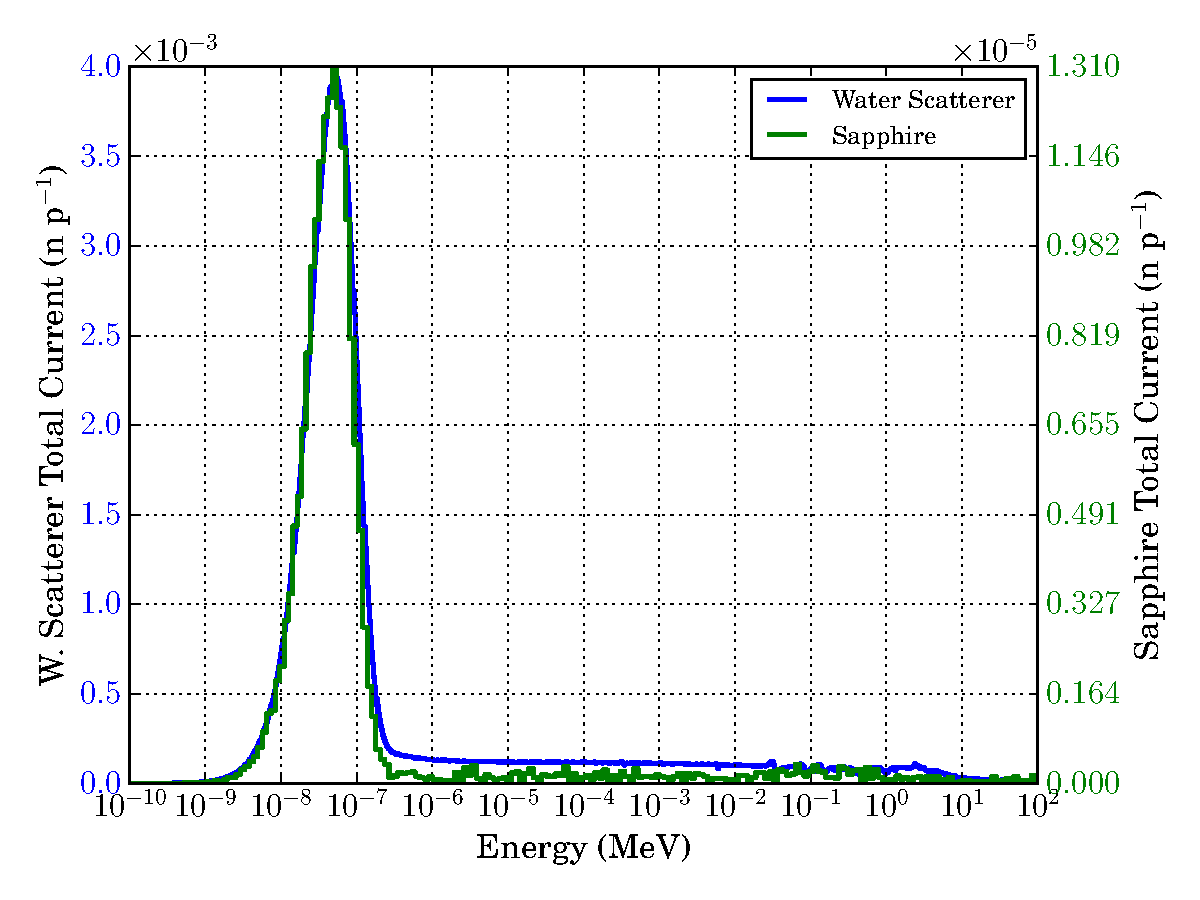
\includegraphics[width=0.7\linewidth]{specs.pdf}\\[1ex]          
            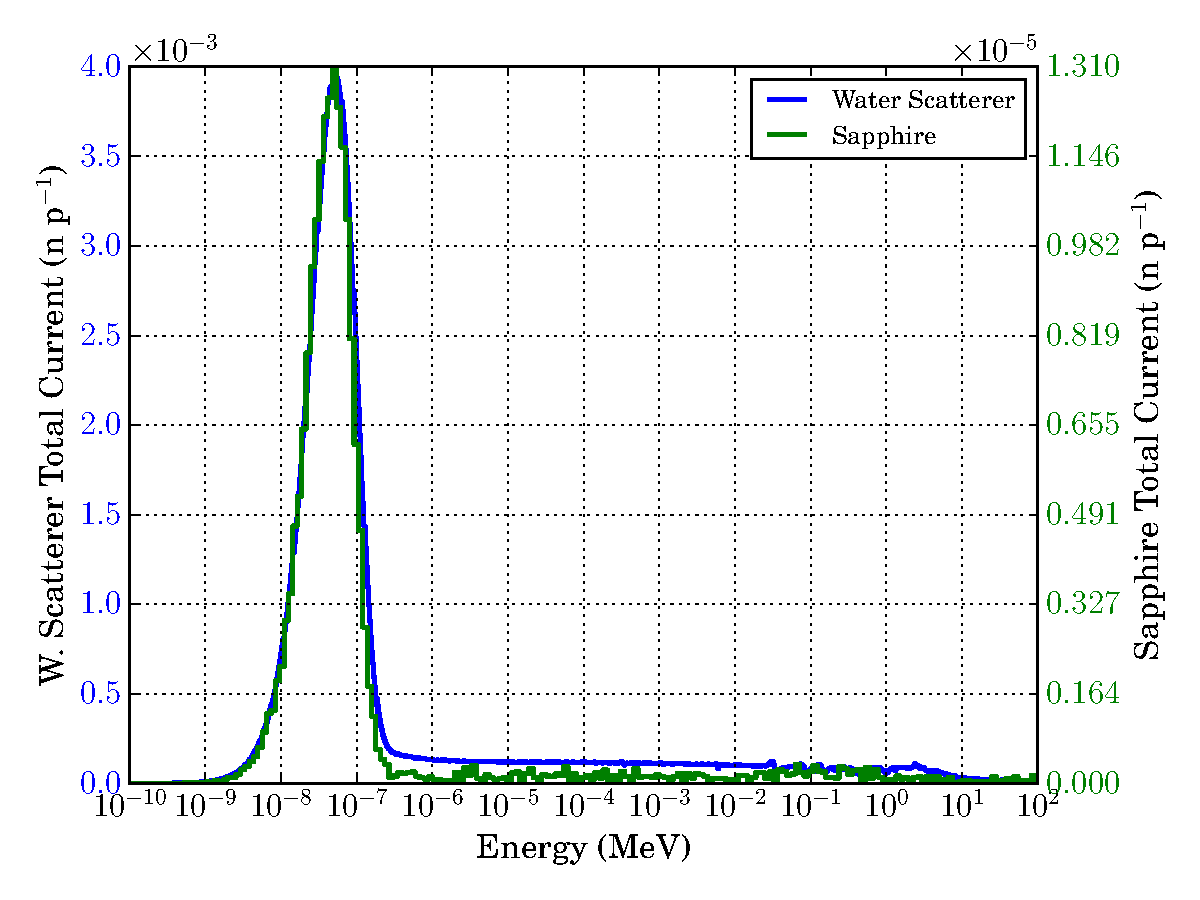
\includegraphics[width=0.7\linewidth]{specs.pdf}\\[1ex]          
          \end{column}
        \end{columns}

      \end{block}

      %%%%%%%%%%%%%%%%%%%%%%%%%%%%%%%%%%%%%%%%%%%%%%%%%%%%%%%%%%%%%%%%%%%%%%%%%%%%%%%%%%%%%%%%%%%%%%%%%%%%%%%%%%%%

    \end{column}
    \begin{column}{.3\linewidth}
      \begin{block}{System Overview}
        \vfill
        \noindent{\textbf{Visual Modeling (VM)}}
        \begin{itemize}
        \item related to the acoustic model in ASR
        \item HMM based, with separate GMMs, globally pooled diag. covariance matrix
        \item monophone whole-word models
        \item pronunciation handling
        \end{itemize}

        \vskip1ex
        \noindent{\textbf{Language Modeling (LM)}}
        \begin{itemize}
        \item according to ASR: LM should have a greater weight than the VM
        \item trigram LM using the SRILM toolkit, with modified Kneser-Ney discounting with interpolation
        \end{itemize}

        \vskip1ex
        \begin{columns}[t]
          \begin{column}{.5\linewidth}
            \noindent{\hskip1cm\textbf{Features}}\par
            \begin{itemize}
            \item \alert{appearance-based image features}: for baseline system
              \begin{itemize}
              \item thumb\-nails of video se\-quen\-ce fra\-mes (intensity images scaled to 32x32 pixels)
              \item give a global description of all (manual and non-manual) features proposed in linguistic research
              \end{itemize}
            \item \alert{manual features}: 
              \begin{itemize}
              \item dominant hand \alert{tracking}: hand position,
                hand velocity, and hand trajectory features
              \end{itemize}
            \end{itemize}
          \end{column}
          \begin{column}{.5\linewidth}
            \vskip0ex
            %%%%%%%%%%%%%%%%%%%%%%%%%%%%%%%%%%%%%%%%%%%%%%%%%%%%%%%
            \centering
            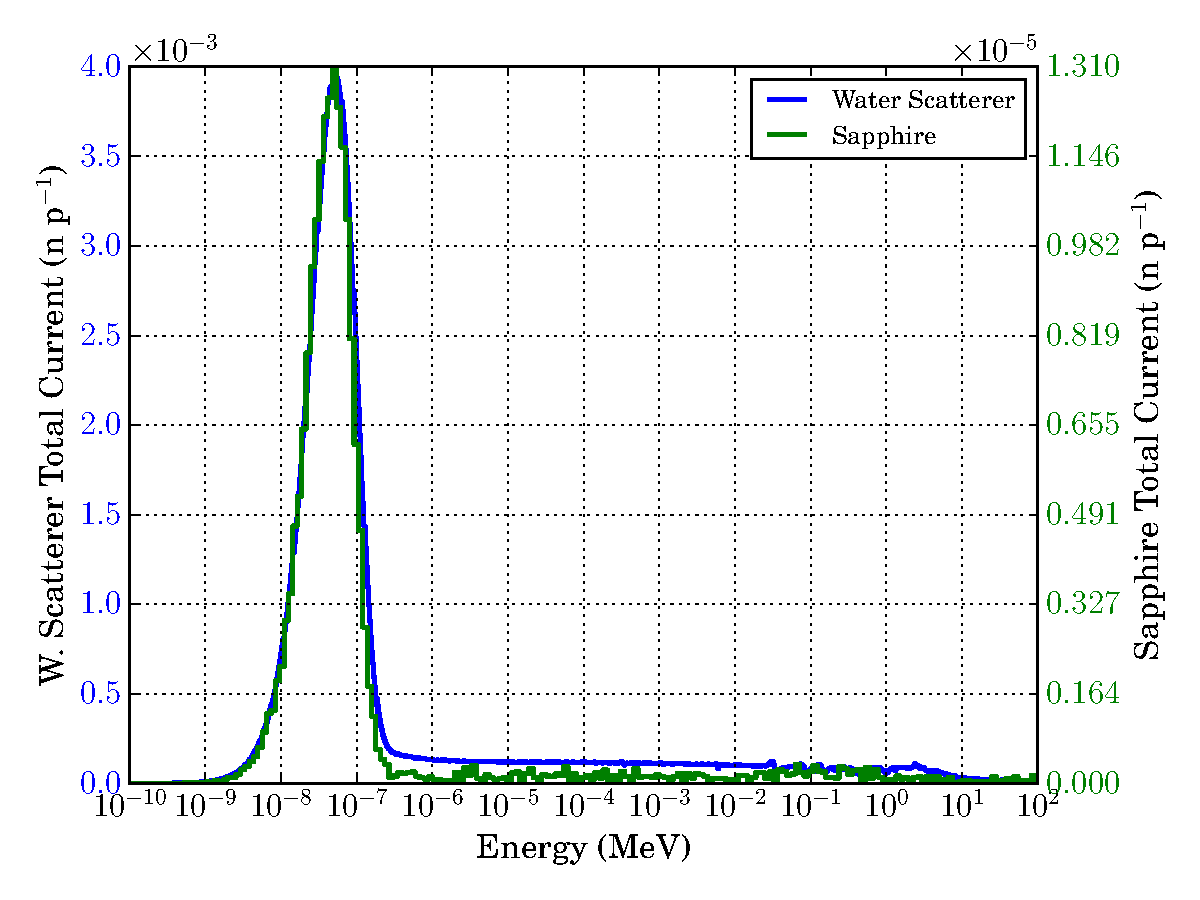
\includegraphics[height=0.33\linewidth]{specs.pdf}
            \quad\quad
            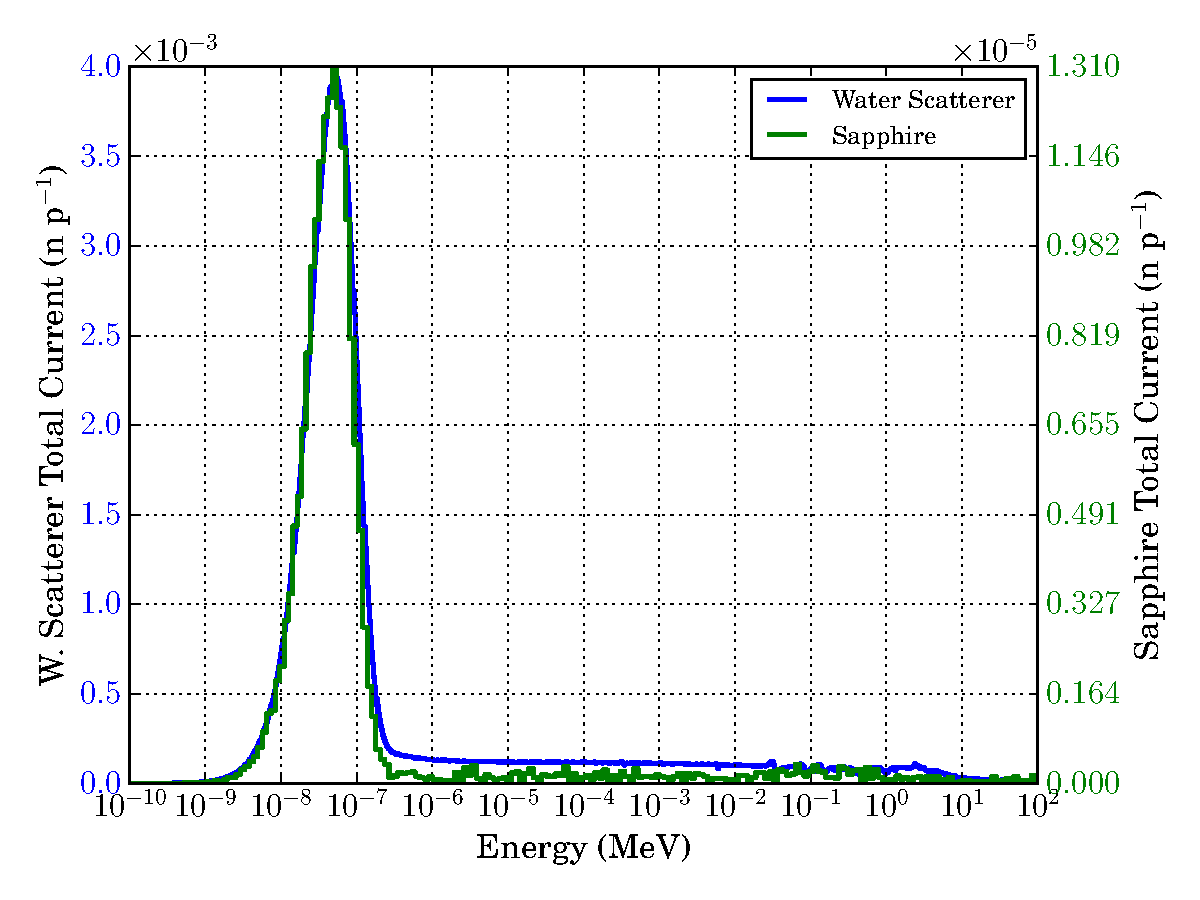
\includegraphics[height=0.33\linewidth]{specs.pdf}
            \vskip3ex
            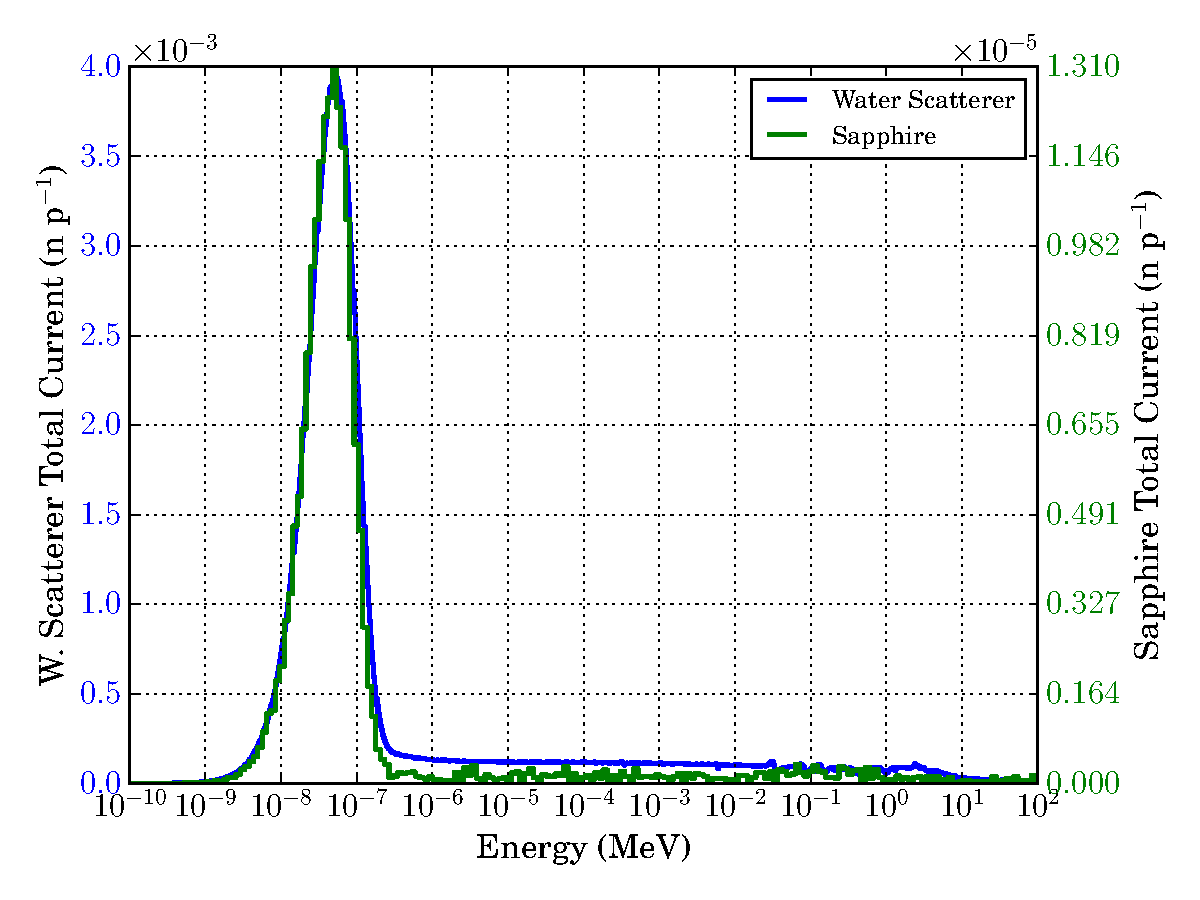
\includegraphics[height=0.4\linewidth]{specs.pdf}
            \quad
            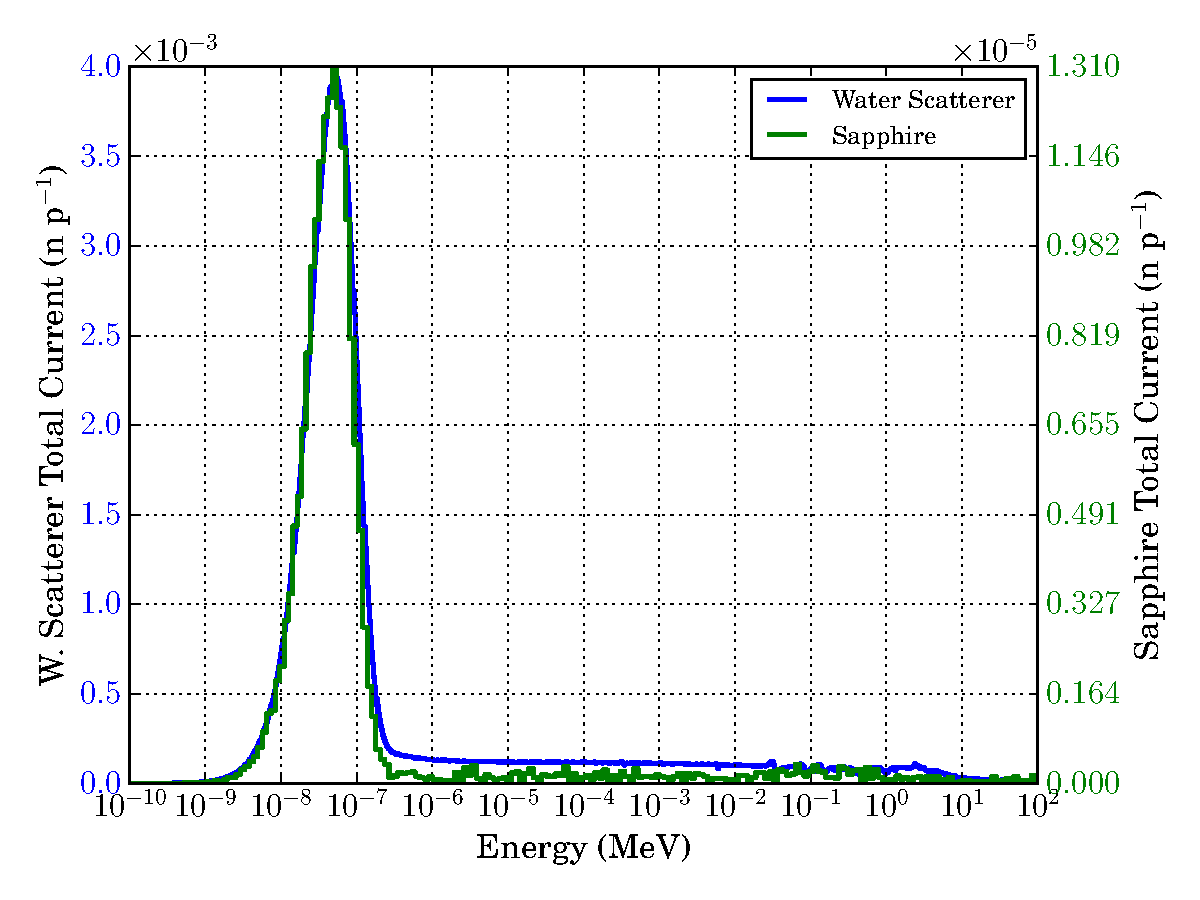
\includegraphics[height=0.4\linewidth]{specs.pdf}
            %%%%%%%%%%%%%%%%%%%%%%%%%%%%%%%%%%%%%%%%%%%%%%%%%%%%%%%
          \end{column}
        \end{columns}
      \end{block}

      \begin{block}{Feature Selection and Model Combination}
        \begin{columns}[T]
          \begin{column}{.35\linewidth}
            \noindent{\hskip1cm\textbf{Feature Selection}}\par
            \begin{itemize}
            \item \alert{concatenation} of appearance-based and manual features
            \item \alert{sliding window} for context modeling
            \item \alert{dimensionality reduction} by PCA and/or LDA
            \end{itemize}
          \end{column}
          \begin{column}{.65\linewidth}
            \raggedleft
            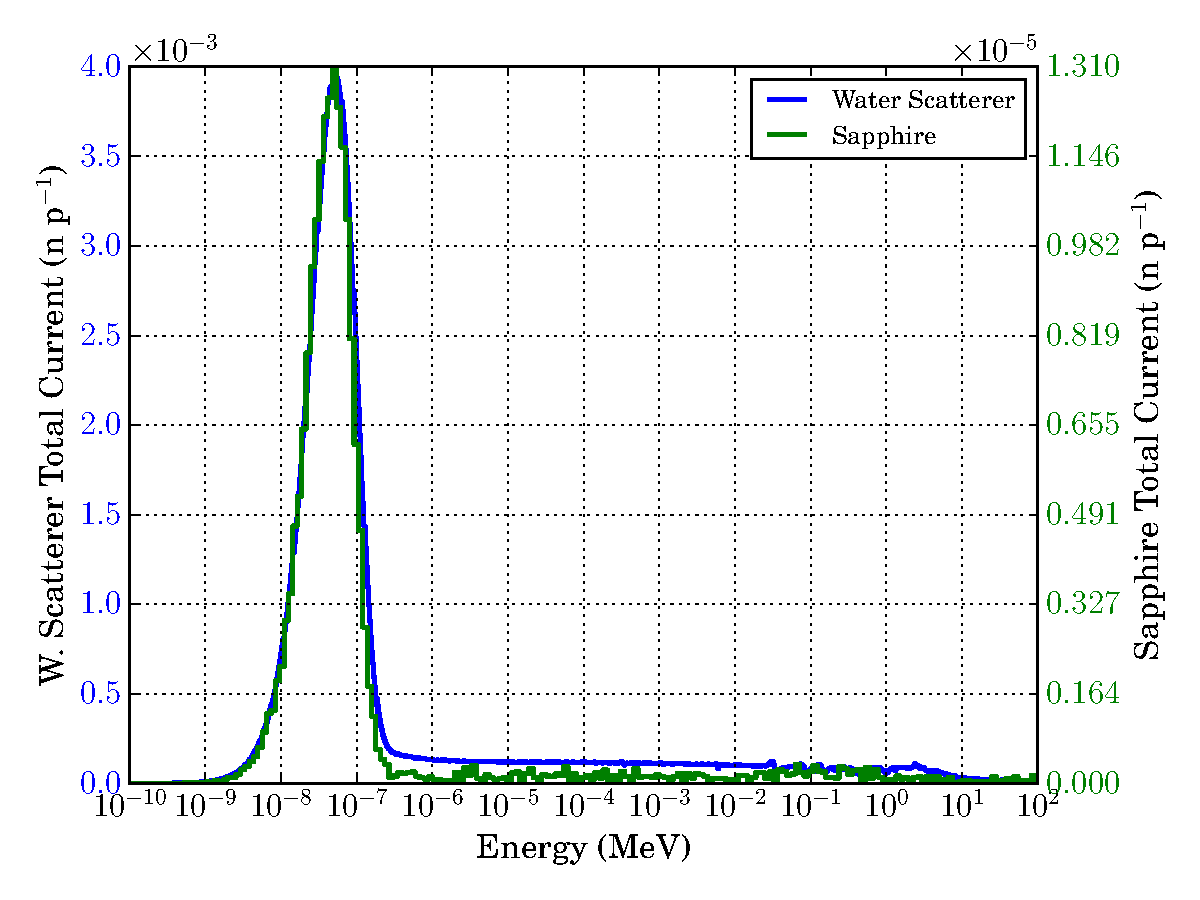
\includegraphics[width=.95\linewidth]{specs.pdf}%
          \end{column}
        \end{columns}

        \vskip5ex
        \begin{columns}[T]
          \begin{column}{.35\linewidth}
            \noindent{\hskip1cm\textbf{Model Combination}}\par
            \begin{itemize}
            \item \alert{log-linear combination} of independently
              trained models
            \item profit from independent alignments (\eg performing well for long and short words)
            \item profit from different feature extraction approaches
            \end{itemize}
          \end{column}
          \begin{column}{.65\linewidth}
            \raggedleft
            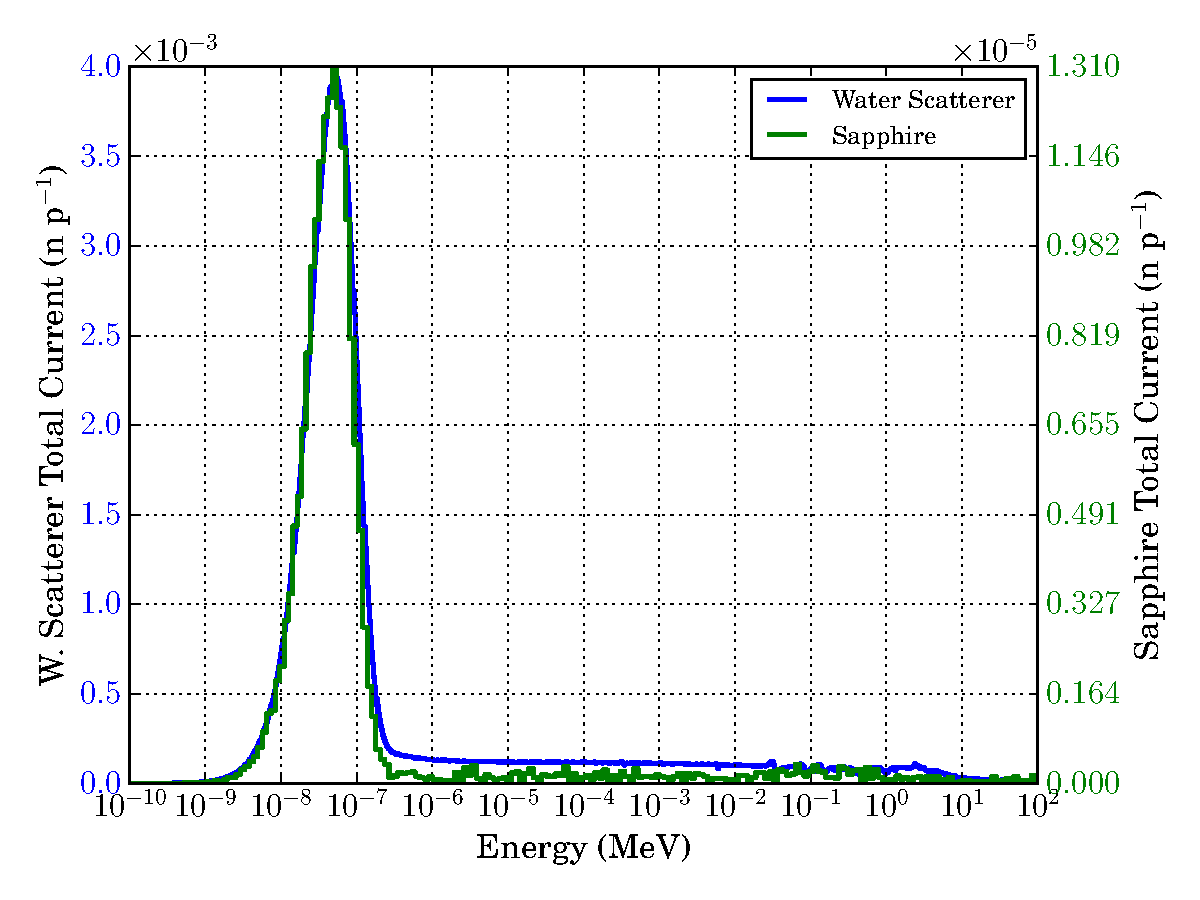
\includegraphics[width=\linewidth]{specs.pdf}
          \end{column}
        \end{columns}


        %%%%%%%%%%%%%%%%%%%%%%%%%%%%%%%%%%%%%%%%%%%%%%%%%%%%%%%
      \end{block}

    \end{column}

    %%%%%%%%%%%%%%%%%%%%%%%%%%%%%%%
    
    \begin{column}{.3\linewidth}

      \begin{block}{Experimental Results}
        %%%%%%%%%%%%%%%%%%%%%%%%%%%%%%%%%%%%%%%%%%%%%%%%%%%%%%%
        \centering
        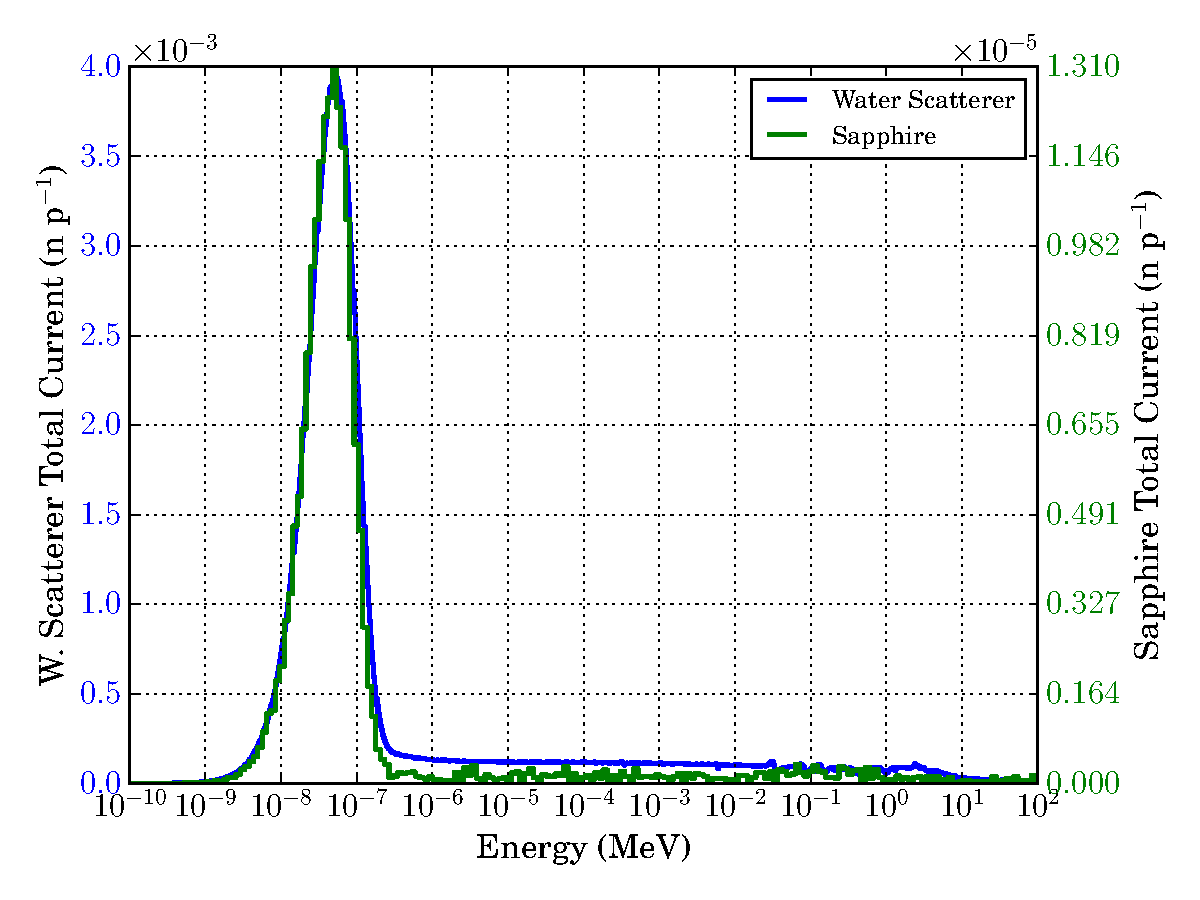
\includegraphics[width=0.33\linewidth]{specs.pdf}%
        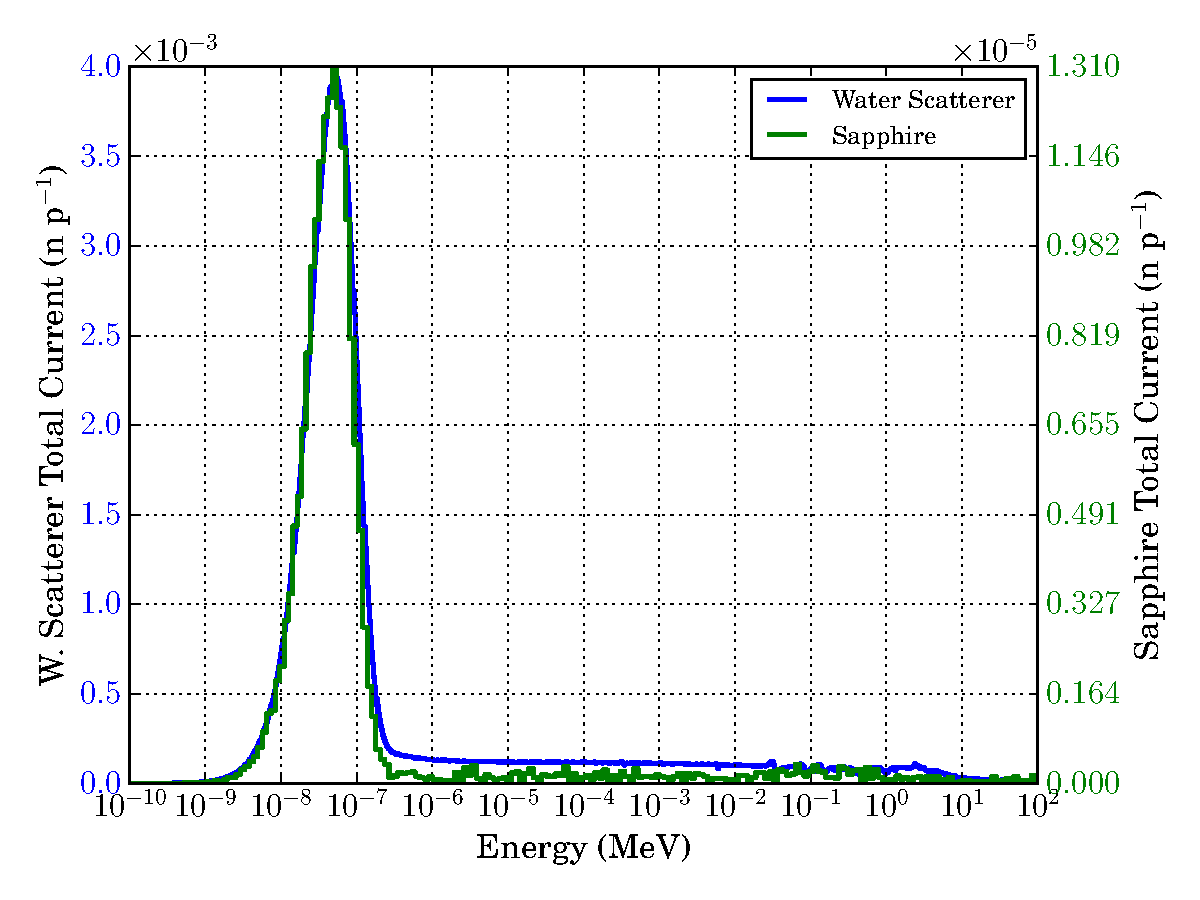
\includegraphics[width=0.33\linewidth]{specs.pdf}%
        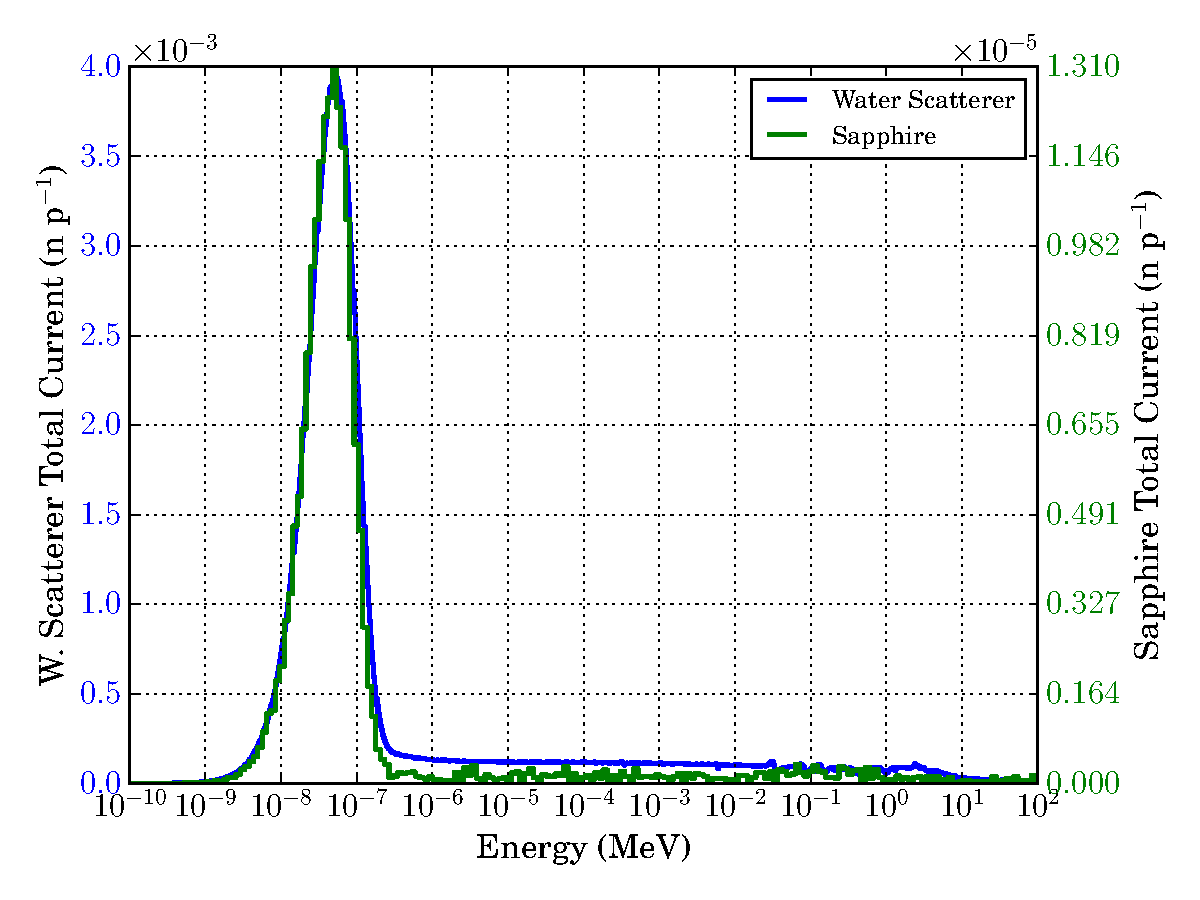
\includegraphics[width=0.33\linewidth]{specs.pdf}%
        %%%%%%%%%%%%%%%%%%%%%%%%%%%%%%%%%%%%%%%%%%%%%%%%%%%%%%%

        %%%%%%%%%%%%%%%%%%%%%%%%%%%%%%%%%%%%%%%%%%%%%%%%%%%%%%%
        \begin{table}
        \end{table}
      \end{block}
      
      \vskip-2ex
      \begin{columns}[t]
        ~~
        \begin{column}{.57\linewidth}
          \begin{block}{Example Results}   
            \noindent{\hskip1cm\textbf{Correct Examples}}        
            \hrule
            \begin{tabular}{@{}>{\small}c@{}>{\small}c@{}>{\small}c@{}>{\small}c}
              IX-1P & \ \ FIND & \ \ SOMETHING-ONE & \ \ BOOK\\
              \textcolor{black}{IX-1P} & \ \ \textcolor{black}{FIND} & \ \ \textcolor{black}{SOMETHING-ONE} & \ \ \textcolor{black}{BOOK}
            \end{tabular}
            \hrule
            \begin{tabular}{@{}>{\small}c@{}>{\small}c@{}>{\small}c@{}>{\small}c@{}>{\small}c@{}>{\small}c@{}>{\small}c@{}>{\small}c}
              JOHN & \ \ FISH & \ \ WONT & \ \ EAT & \ \ BUT & \ \ CAN & \ \ EAT & \ \ CHICKEN\\
              \textcolor{black}{JOHN} & \ \ \textcolor{black}{FISH} & \ \ \textcolor{black}{WONT} & \ \ \textcolor{black}{EAT} & \ \ \textcolor{black}{BUT} & \ \ \textcolor{black}{CAN} & \ \ \textcolor{black}{EAT} & \ \ \textcolor{black}{CHICKEN}
            \end{tabular}
            \hrule
            \begin{tabular}{@{}>{\small}c@{}>{\small}c@{}>{\small}c}
              LOVE & \ \ JOHN & \ \ WHO\\
              \textcolor{black}{LOVE} & \ \ \textcolor{black}{JOHN} & \ \ \textcolor{black}{WHO}
            \end{tabular}
            \hrule
            \begin{tabular}{@{}>{\small}c@{}>{\small}c@{}>{\small}c@{}>{\small}c@{}>{\small}c}
              JOHN & \ \ BUY & \ \ YESTERDAY & \ \ WHAT & \ \ BOOK\\
              \textcolor{black}{JOHN} & \ \ \textcolor{black}{BUY} & \ \ \textcolor{black}{YESTERDAY} & \ \ \textcolor{black}{WHAT} & \ \ \textcolor{black}{BOOK}
            \end{tabular}
            \hrule          
            \vskip2ex
            \noindent{\hskip1cm\textbf{Incorrect Examples}}\par                              
            \hrule
            \begin{tabular}{@{}>{\small}c@{}>{\small}c@{}>{\small}c@{}>{\small}c@{}>{\small}c@{}>{\small}c}
              MARY & \ \ VEGETABLE & \ \ KNOW & \ \ IX & \ \ LIKE & \ \ CORN\\
              \textcolor{black}{MARY} & \ \ \textcolor{black}{VEGETABLE} & \ \ \textcolor{black}{KNOW} & \ \ \textcolor{black}{IX} & \ \ \textcolor{black}{LIKE} & \ \ \textcolor{red}{MARY}
            \end{tabular}
            \hrule
            \begin{tabular}{@{}>{\small}c@{}>{\small}c@{}>{\small}c@{}>{\small}c@{}>{\small}c@{}>{\small}c@{}>{\small}c}
              JOHN & \ \ IX & \ \ GIVE & \ \ MAN & \ \ IX & \ \ NEW & \ \ COAT\\
              \textcolor{black}{JOHN} & \ \ \textcolor{black}{IX} & \ \ \textcolor{red}{WOMAN} & \ \ \textcolor{black}{\underline{\phantom{MAN}}} & \ \ \textcolor{black}{\underline{\phantom{IX}}} & \ \ \textcolor{black}{NEW} & \ \ \textcolor{black}{COAT}
            \end{tabular}
            \hrule
            \begin{tabular}{@{}>{\small}c@{}>{\small}c@{}>{\small}c@{}>{\small}c}
              & \ \ LIKE & \ \ CHOCOLATE & \ \ WHO\\
              \textcolor{green}{JOHN} & \ \ \textcolor{black}{LIKE} & \ \ \textcolor{black}{CHOCOLATE} & \ \ \textcolor{black}{WHO}
            \end{tabular}
            \hrule
            \begin{tabular}{@{}>{\small}c@{}>{\small}c@{}>{\small}c@{}>{\small}c@{}>{\small}c}
              JOHN & \ \ [UNKNOWN] & \ \  & \ \ BUY & \ \ HOUSE\\
              \textcolor{black}{JOHN} & \ \ \textcolor{red}{FUTURE} & \ \ \textcolor{green}{NOT} & \ \ \textcolor{black}{BUY} & \ \ \textcolor{black}{HOUSE}
            \end{tabular}
            \hrule
            \vspace{-1ex}            
          \end{block}
        \end{column}
        ~
        \begin{column}{.4\linewidth}
          \begin{block}{RWTH-BOSTON-104 Database}   
            %%%%%%%%%%%%%%%%%%%%%%%%%%%%%%%%%%%%%%%%%%%%%%%%%%%%%%
            \noindent{\hskip1cm\textbf{Corpus Statistics}}        
            \begin{table}
              \centering
              %\footnotesize
              %\caption{Corpus Statistics}
              \begin{tabular}{@{} p{.5\linewidth}  r r @{}}
                \toprule
                                 & Training   &  Test \\
                \midrule
                sentences        & 161        &  40   \\
                running words    & 710        & 178   \\
                frames           & 12422      & 3324  \\
                vocabulary       & 103        &  65   \\
                singletons       &  27        &   9   \\
                OOV              & -          &   1   \\
                \bottomrule
              \end{tabular}
            \end{table}
            \vskip2ex
            %%%%%%%%%%%%%%%%%%%%%%%%%%%%%%%%%%%%%%%%%%%%%%%%%%%%%%
            \noindent{\hskip1cm\textbf{LM Perplexities}}        
            \begin{table}
              \centering
              %\caption{}
              \begin{tabular}{@{} p{.8\linewidth} r @{}}
                \toprule
                LM type     & $PP$ \\
                \hline
                zerogram    & 106.0 \\
                unigram     & 36.8 \\
                bigram      & 6.7 \\
                trigram     & 4.7 \\
                \bottomrule
              \end{tabular}
            \end{table}
            %%%%%%%%%%%%%%%%%%%%%%%%%%%%%%%%%%%%%%%%%%%%%%%%%%%%%%%
            \vskip2ex
            Database is publicly available
          \end{block}
        \end{column}
      \end{columns}
                
      \begin{block}{Conclusion}
        \begin{itemize}
        \item LVSR system is suitable for vision-based continuous sign language recognition
        \item many of the principles known from ASR can directly be transfered 
        \item important for ASLR: temporal contexts, pronunciation handling, language modelling, and model combination
        \item \alert{outlook:} connection of recognizer output to a
          statistical machine translation system achieved promising
          translation results
        \end{itemize}
        \vspace{-1ex}
      \end{block}
%%%%%%%%%%%%%%%%%%%%%%%%%%%%%%%%%%%%%%%%%%%%%%%%%%%%%%%

    \end{column}
  \end{columns}
\end{frame}

\end{document}


%%%%%%%%%%%%%%%%%%%%%%%%%%%%%%%%%%%%%%%%%%%%%%%%%%%%%%%%%%%%%%%%%%%%%%%%%%%%%%%%%%%%%%%%%%%%%%%%%%%%
%%% Local Variables: 
%%% mode: latex
%%% TeX-PDF-mode: t
%%% End: 